\documentclass{article}
\usepackage{amsmath, amsfonts, tcolorbox, import}
\subimport*{./}{macro}
\setlength\parindent{0px}
\tcbset{
  answerbox/.style={
    colback=gray!10,       % light gray background
    colframe=black!40,     % dark gray border
    boxrule=0.4mm,
    arc=1mm,
    left=1mm,
    right=1mm,
    top=1mm,
    bottom=1mm,
    width=\textwidth,
    before skip=5pt,
    after skip=10pt,
  }
}

\begin{document}
\setcounter{aprob}{0}
\setcounter{bprob}{0}
\title{Homework \#0}
\author{
    \normalsize{CSE 446: Machine Learning}\\
    \normalsize{Ananya Shreya Soni}\\
    \normalsize{Date: \textbf{Wednesday} April 9, 2025 11:59pm}\\
}
\date{{}}
\maketitle



% Start of Problems:

\section*{Probability and Statistics}
\begin{aprob}
    \points{2} (From Murphy Exercise 2.4.) 
    After your yearly checkup, the doctor has bad news and good news. 
    The bad news is that you tested positive for a serious disease, and that the test is 99\% accurate (i.e., the probability of testing positive given that you have the disease is 0.99, as is the probability of testing negative given that you don't have the disease).
    The good news is that this is a rare disease, striking only one in 10,000 people.
    What are the chances that you actually have the disease?
    \begin{tcolorbox}[colback=lightgray!10!white, colframe=black, title=A1]
        \begin{itemize}
            \item Let $P$ be the event of testing positive.
            \item Let $D$ be the event of having the disease.
        \end{itemize}
        \textbf{Given:}
        \[
        \mathbb{P}(P \mid D) = 0.99, \quad \mathbb{P}(\neg P \mid \neg D) = 0.99, \quad \mathbb{P}(D) = \frac{1}{10,000}
        \]
        \[
        \mathbb{P}(P \mid \neg D) = 1 - \mathbb{P}(\neg P \mid \neg D) = 0.01
        \]
        \textbf{We want to find:} $\mathbb{P}(D \mid P)$
        \textbf{By Bayes’ Theorem:}
        \[
        \mathbb{P}(D \mid P) = 
        \frac{\mathbb{P}(P \mid D) \cdot \mathbb{P}(D)}{\mathbb{P}(P)}
        \]
        \textbf{Using the Law of Total Probability:}
        \[
        \mathbb{P}(P) = \mathbb{P}(P \mid D) \cdot \mathbb{P}(D) + \mathbb{P}(P \mid \neg D) \cdot \mathbb{P}(\neg D)
        \]
        \[
        \mathbb{P}(D \mid P) =
        \frac{0.99 \cdot \frac{1}{10,000}}{0.99 \cdot \frac{1}{10,000} + 0.01 \cdot \left(1 - \frac{1}{10,000}\right)}
        \]
        \[
        \approx 0.0098
        \]
        \textbf{Therefore, the probability that you actually have the disease given a positive test result is approximately 0.98\%.}
    \end{tcolorbox}
\end{aprob}

\begin{aprob}
    For any two random variables $X,Y$ the \emph{covariance} is defined as $\Cov{X}{Y}=\E{(X-\E{X})(Y-\E{Y})}$. 
    You may assume $X$ and $Y$ take on a discrete values if you find that is easier to work with.
    \begin{enumerate}
        \item \points{1} If $\E{Y\given X=x} = x$ show that $\Cov{X}{Y} = \E{\round{X-\E{X}}^2}$.  
        \item \points{1} If $X, Y$ are independent show that $\Cov{X}{Y}=0$.
    \end{enumerate}

    \begin{tcolorbox}[colback=lightgray!10!white, colframe=black, title=A2.a]
        \[
        \textbf{Lemma 1: }
        \mathbb{E}[Y|X=x] = \sum_{y \in \Omega_Y} y \cdot \mathbb{P}_{Y|X}(y|x) = x \quad \text{(by given and definition of conditional expectation)}
        \]
        \textbf{Lemma 2: } $\mathbb{E}[X] = \mathbb{E}[Y]$:
        \begin{align*}
        \mathbb{E}[Y] &= \sum_{x \in \Omega_X} \mathbb{E}[Y|X=x] \cdot \mathbb{P}_X(x) \quad \text{(by Law of Total Expectation)} \\
        &= \sum_{x \in \Omega_X} x \cdot \mathbb{P}_X(x) \quad \text{(by Lemma 1)}\\
        &= \mathbb{E}[X] \quad
        \end{align*}
        \textbf{Lemma 3: } $\mathbb{E}[XY] = \mathbb{E}[X^2]$
        \begin{align*}
        \mathbb{E}[XY] &= \sum_{x,y \in \Omega_{X,Y}} xy \cdot \mathbb{P}_{X,Y}(x,y) \quad \text{(by definintion of expectation)} \\
        &= \sum_{x,y \in \Omega_{X,Y}} xy \cdot \mathbb{P}_{Y|X}(y|x) \cdot \mathbb{P}_X(x) \\
        &= \sum_{x \in \Omega_X} x^2 \cdot \mathbb{P}_X(x) \quad \text{(by Lemma 1)}\\
        &= \mathbb{E}[X^2] \quad \text{(by definintion of expectation)}
        \end{align*}
        \textbf{Lemma 4: } $\mathbb{E}[Y\mathbb{E}[X]] = \mathbb{E}[X\mathbb{E}[X]]$
        \begin{align*}
        \mathbb{E}[Y\mathbb{E}[X]] &= \sum_{x \in \Omega_X} \mathbb{E}[Y|X=x] \cdot \mathbb{P}_X(x) \cdot \mathbb{E}[X] \quad \text{(by Law of Total Expectation)}\\
        &= \sum_{x \in \Omega_X} x \cdot \mathbb{E}[X] \cdot _X(x) \quad \text{(by Lemma 1)} \\
        &= \mathbb{E}[X\mathbb{E}[X]] \quad \text{(by definition of expectation)}
        \end{align*}
        \begin{align*}
        \textbf{Cov}(X, Y) &= \mathbb{E}[(X - \mathbb{E}[X])(Y - \mathbb{E}[Y])] \quad \text{(by definintion of covariance)} \\
        &= \mathbb{E}[XY - Y\mathbb{E}[X] - X\mathbb{E}[Y] + \mathbb{E}[X]\mathbb{E}[Y]] \\
        &= \mathbb{E}[XY] - \mathbb{E}[Y\mathbb{E}[X]] - \mathbb{E}[X\mathbb{E}[Y]] + \mathbb{E}[X]\mathbb{E}[Y] \quad \text{(by Linearity of Expectation)} \\
        &= \mathbb{E}[X^2] - \mathbb{E}[X\mathbb{E}[X]] - \mathbb{E}[X\mathbb{E}[X]] + \mathbb{E}[X]\mathbb{E}[X] \quad \text{(by Lemmas 2, 3, and 4)} \\
        &= \mathbb{E}[X^2] - 2\mathbb{E}[X\mathbb{E}[X]] + \mathbb{E}[X]^2 \\
        &= \mathbb{E}[X^2 - 2X\mathbb{E}[X] + \mathbb{E}[X]^2] \quad \text{(by Linearity of Expectation)} \\
        &= \mathbb{E}[(X - \mathbb{E}[X])^2]
        \end{align*}
        \end{tcolorbox}
        \begin{tcolorbox}[colback=lightgray!10!white, colframe=black, title=A2.b]
        If $X$ and $Y$ are independent, then
        \[
        \mathbb{E}[XY] = \mathbb{E}[X] \cdot \mathbb{E}[Y] \quad \text{(by Independence)}
        \]
        \begin{align*}
        \text{Cov}(X,Y) &= \mathbb{E}[XY] - \mathbb{E}[X] \cdot \mathbb{E}[Y] \quad \text{(by definintion of covariance)}\\
        &= \mathbb{E}[X] \cdot \mathbb{E}[Y] - \mathbb{E}[X] \cdot \mathbb{E}[Y] \\
        &= 0
        \end{align*}
        \end{tcolorbox}
\end{aprob}

\begin{aprob}
    Let $X$ and $Y$ be independent random variables with PDFs given by $f$ and $g$, respectively.
    Let $h$ be the PDF of the random variable $Z = X+Y$.
    \begin{enumerate}
        \item \points{1} Show that $h(z) = \int_{-\infty}^\infty f(x) g( z - x ) \diff x $.  (If you are more comfortable with discrete probabilities, you can instead derive an analogous expression for the discrete case,  and then you should give a one sentence explanation as to why your expression is analogous to the continuous case.)
        \item \optional \color{red}{If $X$ and $Y$ are both independent and uniformly distributed on $[0,1]$ (i.e. $f(x)=g(x)=1$ for $x \in [0,1]$ and $0$ otherwise) what is $h$, the PDF of $Z=X+Y$?}
    \end{enumerate}
    \begin{tcolorbox}[colback=lightgray!10!white, colframe=black, title=A3]
        \textbf{Determine the PDF of $Z$:} \\
        Let $F_Z(z) = \mathbb{P}(Z \leq z)$ be the CDF of $Z = X+Y$. Then:
        \begin{align*}
        F_Z(z) &= \mathbb{P}(X + Y \leq z) \quad \text{(by definintion of Z)} \\
        &= \int_{x \in \Omega_X} \mathbb{P}(x + Y \leq z \mid X = x) f_X(x) \, dx \quad \text{(by the Law of Total Probability and given $X$ = $x$)} \\
        &= \int_{x \in \Omega_X} \mathbb{P}(Y \leq z - x \mid X = x) f_X(x) \, dx \\
        &= \int_{x \in \Omega_X} \mathbb{P}(Y \leq z - x) f_X(x) \, dx \quad \text{(since X and Y are Independent)} \\
        &= \int_{x \in \Omega_X} F_Y(z - x) f_X(x) \, dx \quad \text{(by definition of CDF of Y)}
        \end{align*}
        Differentiate the CDF $F_Z(z)$ with respect to $z$ to get the PDF of $Z$:
        \[
        h(z) = f_Z(z) = \frac{d}{dz} F_Z(z) = \int_{x \in \Omega_X} f_X(x) f_Y(z - x) \, dx
        \]
        Therefore the following holds:
        \[
        h(z) = \int_{-\infty}^\infty f(x) g(z - x) \, dx
        \]
    \end{tcolorbox}
\end{aprob}

\begin{aprob}
    Let $X_1, X_2, ..., X_n \sim \mathcal{N}(\mu, \sigma^2)$ be i.i.d random variables. Compute the following:
    \begin{enumerate}
        \item \points{1} $a\in{\mathbb R},b\in{\mathbb R}$ such that $aX_1+b \sim \mathcal{N}(0,1)$.
        \item \points{1} $\E{X_1 + 2X_2}, \Var{X_1 + 2X_2}$.
        \item \points{2} Setting $\widehat{\mu}_n = \frac{1}{n} \sum_{i=1}^n X_i$, the mean and variance of $\sqrt{n}(\widehat{\mu}_n - \mu)$.
    \end{enumerate}
    \begin{tcolorbox}[colback=lightgray!10!white, colframe=black, title=A4.a]
    We are given $X_1 \sim \mathcal{N}(\mu, \sigma^2)$  and $aX_1 + b \sim \mathcal{N}(0,1)$ \\
    \textbf{Solve for $a$ and $b$:} \\
    \vspace{0.5em} \\
    $\mathbb{E}[aX_1 + b] = a\mathbb{E}[X_1] + b \quad \text{(by Linearity of Expectation)}$ \\
    $= a\mu + b = 0$ \\
    \vspace{0.5em} \\
    $\text{Var}(aX_1 + b) = a^2\text{Var}(X_1)$ \\
    $= a^2\sigma^2 = 1$ \\
    \vspace{0.5em} \\
    So we have: $a\mu + b = 0$ and $a^2\sigma^2 = 1$ \\
    \vspace{0.5em} \\
    This gives us: \\
    \[
    \begin{aligned}
    a^2\sigma^2 &= 1 \quad\Rightarrow\quad a = \frac{1}{\sigma} \\
    a\mu + b &= 0  \quad\Rightarrow\quad b = -a\mu \quad\Rightarrow\quad b = -\frac{\mu}{\sigma} \\
    \end{aligned}
    \]
    Therefore: $a = \frac{1}{\sigma}, b = -\frac{\mu}{\sigma}$
    \vspace{0.3cm}
    \end{tcolorbox}
    \begin{tcolorbox}[colback=lightgray!10!white, colframe=black, title=A4.b]
    \begin{align*}
    \mathbb{E}[X_1 + 2X_2] &= \mathbb{E}[X_1 + 2X_2] \\
    &= \mathbb{E}[X_1] + 2\mathbb{E}[X_2] \quad \text{(by Linearity of Expectation)} \\
    &= \mu + 2\mu \\
    &= 3\mu
    \end{align*}
    \begin{align*}
    \text{Var}(X_1 + 2X_2) &= \text{Var}(X_1) + \text{Var}(2X_2) \quad \text{(since } X_1 \text{ and } X_2 \text{ are independent)} \\
    &= \text{Var}(X_1) + 4\text{Var}(X_2) \\
    &= \sigma^2 + 4\sigma^2 \\
    &= 5\sigma^2
    \end{align*}
    \end{tcolorbox}
    \begin{tcolorbox}[colback=lightgray!10!white, colframe=black, title=A4.c]
    Find $\mathbb{E}[\sqrt{n}(\hat{\mu}_n - \mu)]$ and $\text{Var}[\sqrt{n}(\hat{\mu}_n - \mu)]$ and we are given $\hat{\mu}_n = \frac{1}{n}\sum_{i=1}^n X_i$
    \[
    \mathbb{E}[\sqrt{n}(\hat{\mu}_n - \mu)] = \mathbb{E}\left[\sqrt{n}\left(\frac{1}{n}\sum_{i=1}^n X_i - \mu\right)\right] = \sqrt{n}\mathbb{E}\left[\frac{1}{n}\sum_{i=1}^n X_i - \mu\right]
    \]
    \[
    = \sqrt{n}\mathbb{E}\left[\frac{1}{n}\sum_{i=1}^n X_i - \mu\right] = \sqrt{n}\left(\mathbb{E}\left[\frac{1}{n}\sum_{i=1}^n X_i\right] - \mu\right) = \sqrt{n}\left(\frac{1}{n}\sum_{i=1}^n \mu - \mu\right) = \sqrt{n}(\mu - \mu)
    \]
    \[
    = \sqrt{n}(0) = 0
    \]
    \[
    \text{Var}[\sqrt{n}(\hat{\mu}_n - \mu)] = \text{Var}\left(\sqrt{n}\left(\frac{1}{n}\sum_{i=1}^n X_i - \mu\right)\right) = n\text{Var}\left(\frac{1}{n}\sum_{i=1}^n X_i - \mu\right) = n\left(\frac{1}{n}\right)^2\sum_{i=1}^n \text{Var}(X_i)
    \]
    \[
    = \frac{1}{n} \cdot n\sigma^2 = \sigma^2
    \]
    \end{tcolorbox}
\end{aprob}



\section*{Linear Algebra and Vector Calculus}
\begin{aprob}
    Let $A = \begin{bmatrix} 1 & 2 & 1 \\ 1 & 0 & 3 \\ 1 & 1 & 2 \end{bmatrix}$ and $B = \begin{bmatrix} 1 & 2 & 3 \\ 1 & 0 & 1 \\ 1 & 1 & 2 \end{bmatrix}$.
    For each matrix $A$ and $B$:
    \begin{enumerate} 
    	\item \points{2} What is its rank? 
    	\item \points{2} What is a (minimal size) basis for its column span?
    \end{enumerate}
    \begin{tcolorbox}[colback=lightgray!10!white, colframe=black, title=A5]
    \textbf{Find EF of A:} \\
    \vspace{1em} \\
    $A = \begin{bmatrix}
    1 & 2 & 1 \\
    1 & 0 & 3 \\
    1 & 1 & 2
    \end{bmatrix}$
    \vspace{1em} \\
    $\begin{bmatrix}
    1 & 2 & 1 \\
    0 & -2 & 2 \\
    0 & -1 & 1
    \end{bmatrix}$ $R_2 = R_2 - R_1$ \quad $R_3 = R_3 - R_1$
    \vspace{1em} \\
    $\begin{bmatrix}
    1 & 2 & 1 \\
    0 & -2 & 2 \\
    0 & -2 & 2
    \end{bmatrix}$ $R_3 = 2R_3$
    \vspace{1em} \\
    $\begin{bmatrix}
    1 & 2 & 1 \\
    0 & -2 & 2 \\
    0 & 0 & 0
    \end{bmatrix}$ $R_3 = R_3 - R_2$
    \vspace{1em} \\
    \textbf{basis for column span}
    $\left\{\begin{bmatrix} 1 \\ 1 \\ 1 \end{bmatrix}, \begin{bmatrix} 2 \\ 0 \\ 1 \end{bmatrix}\right\}$
    \vspace{1em} \\
    rank = 2 since 2 non-zero rows in EF of A \\
    \vspace{1em} \\
    \textbf{Find EF of B:}
    \vspace{1em} \\
    $B = \begin{bmatrix}
    1 & 2 & 3 \\
    1 & 0 & 1 \\
    1 & 1 & 2
    \end{bmatrix}$
    \vspace{1em} \\
    $\begin{bmatrix}
    1 & 2 & 3 \\
    0 & -2 & -2 \\
    0 & -1 & -1
    \end{bmatrix}$ $R_2 = R_2 - R_1$ \quad $R_3 = R_3 - R_1$
    \vspace{1em} \\
    $\begin{bmatrix}
    1 & 2 & 3 \\
    0 & -2 & -2 \\
    0 & -2 & -2
    \end{bmatrix}$ $R_3 = 2R_3$
    \vspace{1em} \\
    $\begin{bmatrix}
    1 & 2 & 3 \\
    0 & -2 & -2 \\
    0 & 0 & 0
    \end{bmatrix}$ $R_3 = R_3 - R_2$ \\
    \textbf{basis for column span}
    $\left\{\begin{bmatrix} 1 \\ 1 \\ 1 \end{bmatrix}, \begin{bmatrix} 2 \\ 0 \\ 1 \end{bmatrix}\right\}$
    \vspace{1em} \\
    rank = 2 since 2 non-zero rows in EF of B \\
    \vspace{1em} \\
    a) Rank of A and B = 2 \\
    b) Minimal basis for column span of A and B = 
    $\left\{\begin{bmatrix} 1 \\ 1 \\ 1 \end{bmatrix}, \begin{bmatrix} 2 \\ 0 \\ 1 \end{bmatrix}\right\}$
    \end{tcolorbox}
\end{aprob}

\begin{aprob}\label{prob:linsystem}
    Let $A = \begin{bmatrix} 0 & 2 & 4 \\ 2 & 4 & 2 \\ 3 & 3 & 1 \end{bmatrix}$, $b = \begin{bmatrix} -2 & -2 & -4 \end{bmatrix}^\top$, and $c=\begin{bmatrix} 1 & 1 & 1 \end{bmatrix}^\top$.
    \begin{enumerate}
    	\item \points{1} What is $Ac$?
    	\item \points{2} What is the solution to the linear system $Ax = b$?
    \end{enumerate}
    \begin{tcolorbox}[colback=lightgray!10!white, colframe=black, title=A6.a]
    $A\vec{c} = \begin{bmatrix} 0 & 2 & 4 \\ 2 & 4 & 2 \\ 3 & 3 & 1 \end{bmatrix} \times \begin{bmatrix} 1 \\ 1 \\ 1 \end{bmatrix} = \begin{bmatrix} 6 \\ 8 \\ 7 \end{bmatrix}$
    \vspace{1em} \\
    \end{tcolorbox}
    \begin{tcolorbox}[colback=lightgray!10!white, colframe=black, title=A6.b]
    $\begin{bmatrix} 0 & 2 & 4 & | & -2 \\ 2 & 4 & 2 & | & -2 \\ 3 & 3 & 1 & | & -4 \end{bmatrix}$
    \vspace{1em} \\
    $\begin{bmatrix} 0 & 1 & 2 & | & -1 \\ 1 & 2 & 1 & | & -1 \\ 1 & 1 & \frac{1}{3} & | & -\frac{4}{3} \end{bmatrix}$ 
    $R_1 = \frac{1}{2}R_1$ \quad $R_2 = \frac{1}{2}R_2$ \quad $R_3 = \frac{1}{3}R_3$
    \vspace{1em} \\
    $\begin{bmatrix} 1 & 1 & \frac{1}{3} & | & -\frac{4}{3} \\ 1 & 2 & 1 & | & -1 \\ 0 & 1 & 2 & | & -1 \end{bmatrix}$ swap $R_1$ with $R_3$
    \vspace{1em} \\
    $\begin{bmatrix} 1 & 1 & \frac{1}{3} & | & -\frac{4}{3} \\ 0 & 1 & \frac{2}{3} & | & \frac{1}{3} \\ 0 & 1 & 2 & | & -1 \end{bmatrix}$ $R_2 = R_2 - R_1$
    \vspace{1em} \\
    $\begin{bmatrix} 1 & 1 & \frac{1}{3} & | & -\frac{4}{3} \\ 0 & 1 & \frac{2}{3} & | & \frac{1}{3} \\ 0 & 0 & \frac{4}{3} & | & -\frac{4}{3} \end{bmatrix}$ $R_3 = R_3 - R_2$
    \vspace{1em} \\
    $\begin{bmatrix} 1 & 1 & \frac{1}{3} & | & -\frac{4}{3} \\ 0 & 1 & 0 & | & 1 \\ 0 & 0 & \frac{4}{3} & | & -\frac{4}{3} \end{bmatrix}$ $R_2 = -\frac{1}{2}R_3 + R_2$
    \vspace{1em} \\
    $\begin{bmatrix} 1 & 1 & 0 & | & -1 \\ 0 & 1 & 0 & | & 1 \\ 0 & 0 & \frac{4}{3} & | & -\frac{4}{3} \end{bmatrix}$ $R_1 = -\frac{1}{4}R_3 + R_1
    \vspace{1em} \\
    \begin{bmatrix} 1 & 0 & 0 & | & -2 \\ 0 & 1 & 0 & | & 1 \\ 0 & 0 & 1 & | & -1 \end{bmatrix}$ $R_1 = -R_2 + R_1$ \quad $R_3 = \frac{3}{4}R_3$ \\
    \vspace{1em} \\
    \textbf{Final Answer:} \\
    $x_1 = -2 \\ x_2 = 1 \\ x_3 = -1$
    \end{tcolorbox}
\end{aprob}

\begin{aprob} \label{prob:sumvec}
    For possibly non-symmetric $\mat{A}, \mat{B} \in \R^{n \times n}$ and $c \in \R$, let $f(x, y) = x^\top \mat{A} x + y^\top \mat{B} x + c$. Define
    $$\nabla_z f(x,y) = \begin{bmatrix}
        \pderiv{f}{z_1}(x,y) & \pderiv{f}{z_2}(x,y) & \dots & \pderiv{f}{z_n}(x,y)
    \end{bmatrix}^\top \; \in{\mathbb R}^{n}\;.$$  

    \textbf{Note:} If you are unfamiliar with gradients, you may find the resources available on the course website useful. Section 4 of Zico Kolter and Chuong Do's \href{http://www.cs.cmu.edu/~zkolter/course/15-884/linalg-review.pdf}{Linear Algebra Review and Reference} may be particularly helpful.\\
    
    \begin{enumerate}
    	\item \points{2} Explicitly write out the function $f(x, y)$ in terms of the components $A_{i,j}$ and $B_{i,j}$ using appropriate summations over the indices.
    	\item \points{2} What is $\nabla_x f(x,y)$ in terms of the summations over indices \emph{and} vector notation?
    	\item \points{2} What is $\nabla_y f(x,y)$ in terms of the summations over indices \emph{and} vector notation?
    \end{enumerate}
    \begin{tcolorbox}[colback=lightgray!10!white, colframe=black, title=A7.a]
    Write $f(x,y)$ in terms of the components $A_{ij}$ and $B_{ij}$. Note: A and B are both $n \times n$ matrices. \\
    \begin{align*}
    f(x,y) &= x^T A x + y^T B x + c \\
    &= x^T \sum_{j=1}^n A_j x_j + y^T \sum_{j=1}^n B_j x_j + c \\
    &= \sum_{i=1}^n x_i \left( \sum_{j=1}^n A_{ij} x_j \right) + \sum_{i=1}^n y_i \left( \sum_{j=1}^n B_{ij} x_j \right) + c \\
    &= \sum_{i=1}^n \sum_{j=1}^n A_{ij} x_i x_j + \sum_{i=1}^n \sum_{j=1}^n B_{ij} y_i x_j + c  
    \end{align*}
    \end{tcolorbox}
    \begin{tcolorbox}[colback=lightgray!10!white, colframe=black, title=A7.b]
        Find $\nabla_x f(x,y)$ \\     
        Summation notation: For all $k$, $\nabla_x f(x,y)_k = $ \\
        \begin{align*}
        \frac{\partial}{\partial x_k} \left( \sum_{i=1}^n \sum_{j=1}^n A_{ij} x_i x_j + \sum_{i=1}^n \sum_{j=1}^n B_{ij} y_i x_j + c \right)
        \end{align*}
        \begin{align*}
        &= \frac{\partial}{\partial x_k} \left( \sum_{i \neq k} \sum_{j \neq k} A_{ij} x_i x_j + \sum_{j \neq k} A_{kj} x_k x_j + \sum_{i \neq k} A_{ik} x_i x_k + A_{kk} x_k^2 + \sum_{i=1}^n \sum_{j \neq k} B_{ij} y_i x_j + \sum_{i=1}^n B_{ik} y_i x_k + c \right)
        \end{align*}
        \begin{align*}
        &= \sum_{j \neq k} A_{kj} x_j + \sum_{i \neq k} A_{ik} x_i + 2 A_{kk} x_k + \sum_{i=1}^n B_{ik} y_i
        \end{align*}
        \begin{align*}
        &= \sum_{j=1}^n A_{kj} x_j + \sum_{i=1}^n A_{ik} x_i + \sum_{i=1}^n B_{ik} y_i
        \end{align*}
        Vector Notation:
        \begin{align*}
        \frac{\partial}{\partial x} (x^T A x + y^T B x + c)
        &= (A + A^T) x + B^T y
        \end{align*}
\end{tcolorbox}
        
\begin{tcolorbox}[colback=lightgray!10!white, colframe=black, title=A7.c]
    Find $\nabla_y f(x,y)$ \\
    Summation notation: For all $k$, $\nabla_y(f(x,y))_k = $ \\
    \begin{align*}
    \frac{\partial}{\partial y_k} \left( \sum_{i=1}^n \sum_{j=1}^n A_{ij} x_i x_j + \sum_{i=1}^n \sum_{j=1}^n B_{ij} y_i x_j + c \right)
    \end{align*}
    \begin{align*}
    &= \frac{\partial}{\partial y_k} \left( \sum_{i=1}^n \sum_{j=1}^n A_{ij} x_i x_j + \sum_{i \neq k} \sum_{j=1}^n B_{ij} y_i x_j + \sum_{j=1}^n B_{kj} y_k x_j + c \right)
    \end{align*}
    \begin{align*}
    &= \sum_{j=1}^n B_{kj} x_j
    \end{align*}
    Vector Notation:
    \begin{align*}
    \frac{\partial}{\partial y} (x^T A x + y^T B x + c)
    &= B x
    \end{align*}
    \end{tcolorbox}
\end{aprob}
\begin{aprob}\label{prob:matrixtype}
    Show the following:
    \begin{enumerate}
        \item \points{2} Let $g\colon \R \rightarrow \R$ and $v, w \in \R^n$ such that $g(v_i) = w_i$ for $i\in[n]$. Find an expression for $g$ such that $\diag(v)^{-1} = \diag(w)$.
        \item \points{2} Let $\mat{A} \in \R^{n \times n}$ be orthonormal and $x \in \R^n$. 
        An orthonormal matrix is a square matrix whose columns and rows are orthonormal vectors, such that $ \mat{A}\mat{A}^\top = \mat{A}^\top \mat{A} = {\bf I}$ where ${\bf I}$ is the identity matrix. 
        Show that $||\mat{A}x||_2^2 = ||x||_2^2$.
        \item \points{2} Let $\mat{B} \in \R^{n \times n}$ be invertible and symmetric. A symmetric matrix is a square matrix satisfying $\mat{B}=\mat{B}^\top$. Show that $\mat{B}^{-1}$ is also symmetric.
        \item \points{2} Let $\mat{C} \in \R^{n \times n}$ be positive semi-definite (PSD). A positive semi-definite matrix is a symmetric matrix satisfying $x^\top \mat{C} x \geq 0$ for any vector $x\in{\mathbb R}^n$. Show that its eigenvalues are non-negative.
    \end{enumerate}
    \begin{tcolorbox}[colback=lightgray!10!white, colframe=black, title=A8.a]
        From $\diag(v)^{-1} = \diag(w)$, we know that the diagonal elements must satisfy $\frac{1}{v_i} = w_i$ for all $i \in [n]$ because:
        \[
            \diag(v) = \begin{bmatrix} 
            v_1 & 0 & 0 & \cdots & 0 \\
            0 & v_2 & 0 & \cdots & 0 \\
            0 & 0 & \ddots & \cdots & 0 \\
            \vdots & \vdots & \vdots & \ddots & \vdots \\
            0 & 0 & 0 & \cdots & v_n
            \end{bmatrix}
        \]
        \[
            \diag(w) = \begin{bmatrix} 
            w_1 & 0 & 0 & \cdots & 0 \\
            0 & w_2 & 0 & \cdots & 0 \\
            0 & 0 & \ddots & \cdots & 0 \\
            \vdots & \vdots & \vdots & \ddots & \vdots \\
            0 & 0 & 0 & \cdots & w_n
            \end{bmatrix}
        \]
        \[
            \diag(v)^{-1} = \begin{bmatrix} 
            \frac{1}{v_1} & 0 & 0 & \cdots & 0 \\
            0 & \frac{1}{v_2} & 0 & \cdots & 0 \\
            0 & 0 & \ddots & \cdots & 0 \\
            \vdots & \vdots & \vdots & \ddots & \vdots \\
            0 & 0 & 0 & \cdots & \frac{1}{v_n}
            \end{bmatrix}
        \]
        By the property of diagonal matrix inversion, the inverse of a diagonal matrix is obtained by replacing each non-zero diagonal element with its reciprocal. Thus, $[\diag(v)^{-1}]_{i} = \frac{1}{v_i}$.
        Since $g(v_i) = w_i$ and $\diag(v)^{-1} = \diag(w)$, we have $w_i = \frac{1}{v_i}$.
        Therefore, $g(x) = \frac{1}{x}$ for $x \neq 0$ is an expression for $g$ that satisfies the condition.
    \end{tcolorbox}
    \begin{tcolorbox}[colback=lightgray!10!white, colframe=black, title=A8.b]
        Show that $\|\mat{A}x\|_2^2 = \|x\|_2^2$:
        \begin{align*}
        \|\mat{A}x\|_2^2 &= (\mat{A}x)^\top(\mat{A}x) \\
        &= x^\top\mat{A}^\top\mat{A}x \quad \text{(property of transpose)} \\
        &= x^\top\mat{I}x \quad \text{(since $\mat{A}$ is orthonormal, $\mat{A}^\top\mat{A} = \mat{I}$)} \\
        &= x^\top x \\
        &= \|x\|_2^2 \quad \text{(by definition of $l_2$ norm)}
        \end{align*}
        \end{tcolorbox}
    \begin{tcolorbox}[colback=lightgray!10!white, colframe=black, title=A8.c]
        Show $\mat{B}^{-1}$ is symmetric when $\mat{B}$ is symmetric and invertible:
        \begin{align*}
            (\mat{B}^{-1})^\top &= (\mat{B}^\top)^{-1} \quad \text{(property of transpose and inverse)}\\
            &= \mat{B}^{-1} \quad \text{(since $\mat{B}$ is symmetric, $\mat{B}^\top = \mat{B}$)}
        \end{align*}
        Therefore, $(\mat{B}^{-1})^\top = \mat{B}^{-1}$, which means $\mat{B}^{-1}$ is symmetric.
    \end{tcolorbox}

    \begin{tcolorbox}[colback=lightgray!10!white, colframe=black, title=A8.d]
        Show the eigenvalues of a positive semi-definite matrix $\mat{C}$ are non-negative:
            
            We can represent $\mat{C}$ as $\mat{C} = \mat{U}\Lambda\mat{U}^\top$, where $\mat{U}$ is the matrix of eigenvectors of $\mat{C}$ and $\Lambda$ is the diagonal matrix of eigenvalues.
            
            For any vector $x \in \mathbb{R}^n$, we have:
            \begin{align*}
                x^\top\mat{C}x &= x^\top\mat{U}\Lambda\mat{U}^\top x\\
                &= y^\top\Lambda y \quad \text{(let $y = \mat{U}^\top x$)}\\
                &= \sum_{i=1}^n \lambda_i y_i^2
            \end{align*}
            
            Since $\mat{C}$ is positive semi-definite, we know $x^\top\mat{C}x \geq 0$ for all $x \in \mathbb{R}^n$. 
            For the sum $\sum_{i=1}^n \lambda_i y_i^2$ to be non-negative, each eigenvalue $\lambda_i$ must be non-negative because $y_i^2$ is guarenteed to be positive.
            Therefore, all eigenvalues of $\mat{C}$ are non-negative ($>= 0$).
    \end{tcolorbox}
\end{aprob}


\section*{Programming}
\textbf{These problems are  available in a .zip file}, with some starter code. All coding questions in this class will have starter code.
\textbf{Before attempting these problems, you will need to set up a Conda environment that you will use for every assignment in the course. Unzip the HW0-A.zip file and read the instructions in the README file to get started.}

\begin{aprob} \label{prob:sumvecimp}
    For $\nabla_x f(x,y)$ as solved for in Problem \ref{prob:sumvec}:
    \begin{enumerate}
        \item \points{1} \sloppy Using native Python, implement \verb|vanilla_solution| using your \verb|vanilla_matmul| and \verb|vanilla_transpose| functions.
        \item \points{1} Now implement \verb|numpy_version| using NumPy functions.
        \item \points{1} Report the difference in wall-clock time for parts a-b, and discuss reasons for the observed difference.
    \end{enumerate}
    \begin{tcolorbox}[colback=lightgray!10!white, colframe=black, title=A9]
    \begin{center}
        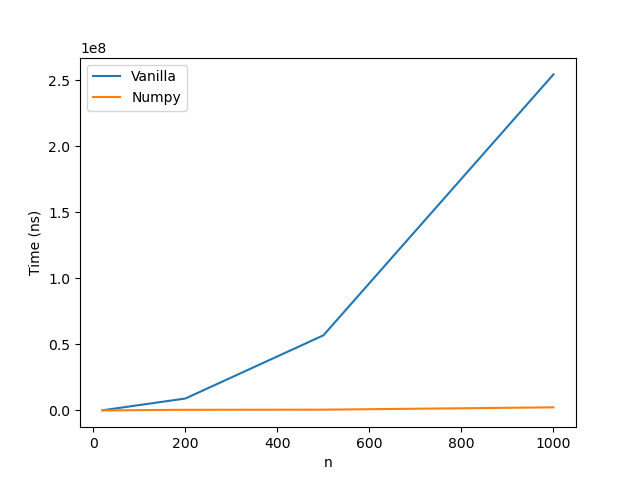
\includegraphics[width=4in]{/Users/ananyasoni/Desktop/cse/cse446/homework/hw0/wall_clock_time_difference_btw_vanilla_and_numpy.png}
    \end{center}
    Time for vanilla implementation: 0.113ms - Time for numpy implementation: 0.018ms = 0.095ms \\
    Time for vanilla implementation: 9.012ms - Time for numpy implementation: 0.468ms = 8.544ms \\
    Time for vanilla implementation: 56.876ms - Time for numpy implementation: 0.574ms = 56.302ms \\
    Time for vanilla implementation: 254.547ms - Time for numpy implementation: 2.337ms = 252.21ms \\

    A reason for the observed difference could be that Numpy does matrix operations like \\
    matrix multiplications much more efficiently than the vanilla nested loop operations. \\
    Additionally, numpy arrays can only store one data type unlike Python lists and Numpy is built with
    C which allows it to do computation much more faster and efficiently than native Python.
    \end{tcolorbox}
\end{aprob}

\begin{aprob}
    Two random variables $X$ and $Y$ have equal  distributions if their CDFs, $F_X$ and $F_Y$, respectively, are equal, i.e. for all $x$, $ \abs{F_X(x) - F_Y(x)} = 0$. 
    The central limit theorem says that the sum of $k$ independent, zero-mean, variance $1/k$ random variables converges to a (standard) Normal distribution as $k$ tends to infinity.  
    We will study this phenomenon empirically (you will use the Python packages NumPy and Matplotlib).  Each of the following subproblems includes a description of how the plots were generated; these have been coded for you. The code is available in the .zip file. In this problem, you will add to our implementation to explore {\bf matplotlib} library, and how the solution depends on $n$ and $k$.
    
    \begin{enumerate}
    \item \points{2}  \label{prob:cltcdf:gaussian} For $i=1,\ldots,n$ let $Z_i \sim \mathcal{N}(0,1)$. Let $x\mapsto F(x)$ denote the true CDF from which each $Z_i$ is drawn (i.e.,  Gaussian). Define  $\widehat{F}_n(x) = \frac{1}{n} \sum_{i=1}^n \1\{ Z_i \leq x\}$ for $x\in\R$ and we will choose $n$ large enough such that, for all $x \in \R$,
    \[
    	\sqrt{\E{\round{\widehat{F}_n(x)-F(x)}^2 }} \leq 0.0025\ .
    \]
    Plot $x\mapsto \widehat{F}_n(x)$ for $x$ ranging from $-3$ to $3$.
    
    \item  \points{2}  Define $Y^{(k)} = \frac{1}{\sqrt{k}} \sum_{i=1}^k B_i$ where each $B_i$ is equal to $-1$ and $1$ with equal probability and the $B_i$'s are independent.
    We know that each $\frac{1}{\sqrt{k}} B_i$ is zero-mean and has variance $1/k$. \label{prob:cltcdf:k} For each $k \in \set{1, 8, 64, 512}$ we will generate $n$ (same as in part a) independent copies $Y^{(k)}$ and plot their empirical CDF on the same plot as part~\ref{prob:cltcdf:gaussian}.
    \end{enumerate}
    Be sure to always label your axes. 
    Your plot should look something like the following (up to styling) (Tip: checkout \texttt{seaborn} for instantly better looking plots.)
    \begin{tcolorbox}[colback=lightgray!10!white, colframe=black, title=A10]
        \begin{center}
            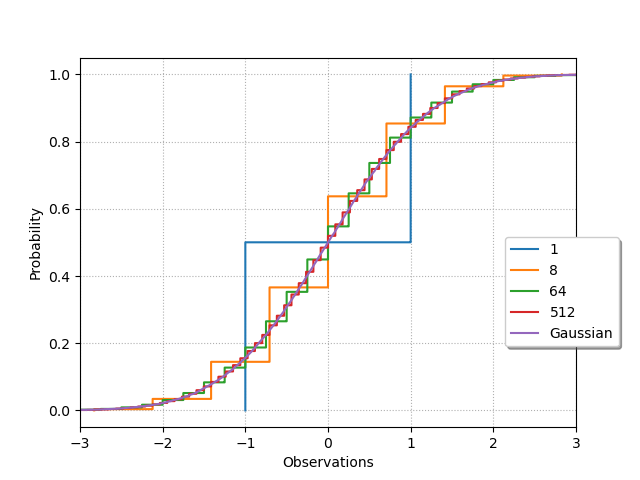
\includegraphics[width=4in]{/Users/ananyasoni/Desktop/cse/cse446/homework/hw0/clt_with_cdf_plot.png}
        \end{center}
        n = 40000

        The empirical CDF increasingly matches the true CDF as k increases.
        The plot visually depicts how as k increases the empirical CDF looks
        more and more like the Gaussian.
    \end{tcolorbox}
\end{aprob}

\end{document}